\documentclass[conference]{IEEEtran-ModifiedForMVIP}
% این فایل از روی نمونه‌ فایل ارائه شده برای کنفرانس مهندسی برق ایران ICEE 
% برای کنفرانس بینایی ماشین و پردازش تصویر ایران به‌روزرسانی شده است.
% فایل منبع و فایلهای ضمیمه‌ی آن با تغییر فایلهایی که توسط آقای دکتر محمود امین طوسی (دانشگاه
% حکیم سبزواری، http://profs.hsu.ac.ir/mamintoosi) در سایت www.parsilatex.com قرار داده 
% شده بودند به دست آمده است. این تغییرات توسط دکتر مسعود بابایی‌زاده داده شده است. 
% البته فایل IEEEtran-ModifiedForICEE.cls در اینجا، 
% اصلاح شده فایل آقای دکتر امین طوسی نیست و مستقیما با دستکاری
% در فایل IEEEtran.cls توسط مسعود بابایی زاده ایجاد شده است.
% برای کنفرانس بینایی ماشین و پردازش تصویر ایران، فایل IEEEtran-ModifiedForICEE.cls 
% با نام IEEEtran-ModifiedForMVIP.cls  تغییر داده شده است.

% مقاله اصلی که این فایل از تغییر فایل آن به دست آمده است، در هفدهمین کنفرانس مهندسی برق 
% ایران در اردیبهشت ۸۸ ارائه شده بوده است.

% شما می‌توانید از این فایل به عنوان یک الگو برای مقالات خود استفاده نمایید.

% برای پردازش پس از یکبار استفاده از xelatex با استفاده از دستور زیر لیست مراجع را تولید نمایید:
% bibtex MVIP_FA_LaTeX_SamplePaper
% و سپس دوبار استفاده از xelatex. 

%%%% فراخوانی پکیج‌های مورد نیاز کاربر %%%%%%%%%%%%%%%%%%%%%%%%%%%%%%%%%%%%%%%%%%%%%%%%%%
\usepackage{setspace}
\usepackage{subfigure}
\usepackage{algorithm}
\usepackage{algorithmic}
\usepackage{graphicx}
\usepackage{amsmath}
%\usepackage[colorlinks, citecolor=blue]{hyperref}

%%%%%%%%%%%%%%%%%%%%%%%%%%%%%%%%%%%%%%%%%%%%%%%%%%%%%%%%%%%%%%%%%%%%%%%%%%%%%%%%%%%%%%%%
%%%% فراخوانی تنظیمات مورد نیاز کنفرانس مهندسی برق ایران و پکیج زی‌پرشین %%%%%%%%%%%%%%%%
% این فایل از روی نمونه‌ فایل ارائه شده برای کنفرانس مهندسی برق ایران ICEE برای کنفرانس بینایی ماشین و پردازش تصویر ایران به‌روزرسانی شده است.
% این فایل شامل تنظیماتی است که قبل از لود شدن پکیج زی‌پرشین باید انجام شوند.
% نویسنده: مسعود بابایی‌زاده
% نسخه 1.0.0
% تاریخ: ۵ مهرماه ۱۳۹۳
%%%%%%%%%%%%%%%%%%%%%%%%%%%%%%%%%%%%%%%%%%
% Start of Page Setup:
\usepackage[top=25mm, bottom=25mm, left=20mm, right=20mm]{geometry}
\setlength{\columnwidth}{82mm}
\setlength{\columnsep}{6mm}
% End of Page Setup
%%%%%%%%%%%%%%%%%%%%%%%%%%%%%%%%%%%%%%%%%%
% یکی از دو روش زیر را انتخاب کنید. گذاشتن حالت «کشیده» باعث می‌شود که تنطیم
% طول خطها بجای اینکه با کم و زیاد کردن فاصله بین کلمات انجام شود، با کشیدن
% کلمات انجام شود. این حالت در فارسی صحیح‌تر و خیلی زیباتر است (برخلاف انگلیسی که کشیدن کلمات
% در آن معنی ندارد و تنطیم طول خطوط فقط با کم و زیاد کردن فاصله بین کلمات صورت
% می‌گیرد). اما با استفاده از حالت «کشیده»، اگر از Acrobat Adobe برای دیدن خروجی پی‌دی‌اف
% استفاده کنید این کشیده‌ها را می‌بینید که چندان زیبا نیست (در نسخه چاپی وجود ندارند).
% اگر می‌خواهید اینها را نبینید در قسمت  Edit->Preferences->PageDisplay گزینه
% Enhance Thin Lines
% را غیرفعال کنید. اما اگر از SumatraPDF برای دیدن فایل پی‌دی‌اف استفاده می‌کنید، تنظیم خاصی
% نیاز نیست.
\usepackage[Kashida]{xepersian}
% \usepackage{xepersian}
% این فایل از روی نمونه‌ فایل ارائه شده برای کنفرانس مهندسی برق ایران ICEE برای کنفرانس بینایی ماشین و پردازش تصویر ایران به‌روزرسانی شده است.
% این فایل شامل تنظیماتی است که بعد از لود شدن پکیج زی‌پرشین باید انجام شوند.
% نویسنده: مسعود بابایی‌زاده
% نسخه 1.0.0
% تاریخ: ۳ مهرماه ۱۳۹۳

%%%%%%%%%%%%%%%%%%%%%%%%%%%%%%%%%%%%%%%%%%
% Font settings

\settextfont[ BoldFont={XB Kayhan Bd.ttf}, BoldItalicFont={XB Kayhan BdIt.ttf}, ItalicFont={XB Kayhan It.ttf},Scale=1.2]{XB Kayhan.ttf}
\setdigitfont[Scale=1.2]{XB Kayhan.ttf}
\setlatintextfont[Scale=1]{Times New Roman}
\defpersianfont\titlefont[Scale=1]{IRTitr.ttf}
\setiranicfont[Scale=1.2]{XB Kayhan It.ttf}				% ایرانیک، خوابیده به چپ

%%%%%%%%%%%%%%%%%%%%%%%%%%%%%%%%%%%%%%%%%%
% تنظیم فاصله خطوط:
% زیاد کردن \baselineskip بر خلاف \baselinestreatch روی محیط ریاضی تاثیری ندارد. اما \baselineskip را باید بعد از \begin{document} زیاد کرد. با توجه به اینکه singlespace برای فرمولهای ریاضی در متن فارسی زیادی کوچک است،‌ پس برای آنکه طبق اعداد بالا فاصله خطوط در فرمولهای 1 برابر و در متن فارسی 1.1 برابر باشد، لازم است که طبق دستور زیر \baselinestreatch برابر 1 قرار داده شود و سپس درون متن و بعد از  \begin{document} باید \baselineskip را 1.1/1.0=1.1 برابر نمود. یعنی:

\renewcommand{\baselinestretch}{1}
%\setlength{\baselineskip}{1.1\baselineskip}   ->  This is inside the text and right after \begin{document}
%برای آنکه کاربر مجبور نباشد دستور بالا را دستی بعد از begin document اضافه کند، دستورات زیر را می‌نویسیم:
\let\olddocument=\document
\let\endolddocument=\enddocument
\renewenvironment{document}{\begin{olddocument}\setlength{\baselineskip}{1.53\baselineskip}}{\end{olddocument}}
%در اینصورت فاصله فرمولها با متن کمی زیاد می‌شود که آن را نیز با دستورات زیر می‌توان حل کرد:
\let\oldequation=\equation
\let\endoldequation=\endequation
% For Yas font
%\renewenvironment{equation}{\vspace{0.2em}\begin{oldequation}}{\vspace{-0.5em}\end{oldequation}\ignorespacesafterend}
% For IRLotus font
\renewenvironment{equation}{\vspace{0.0em}\begin{oldequation}}{\vspace{-0.4em}\end{oldequation}\ignorespacesafterend}


% هبا اعداد بالا در فهرست مطالب و فهرست اشکال و جداول نیز فاصله خطوط زیاد است. که به صورت زیر می‌توان اصلاح کرد (یعنی برای آنها baselineskip را مجددا به عدد قبلی برگرداند، یعنی در معکوس 1.1 که برابر 0.91 می‌شود ضرب کرد):
\let\oldtableofcontents=\tableofcontents
\renewcommand{\tableofcontents}{\begingroup\setlength{\baselineskip}{0.91\baselineskip}\oldtableofcontents\endgroup}

\let\oldlistoffigures=\listoffigures
\renewcommand{\listoffigures}{\begingroup\setlength{\baselineskip}{0.91\baselineskip}\oldlistoffigures\endgroup}

\let\oldlistoftables=\listoftables
\renewcommand{\listoftables}{\begingroup\setlength{\baselineskip}{0.91\baselineskip}\oldlistoftables\endgroup}

% دستور با اعداد بالا، فاصله خطوط در یک متن انگلیسی زیادی  (مثلا فهرست مراجع) بزرگ است. در پایین با تغییر تعریف latin آن را در 0.91 ضرب کرده‌ام:
\let\oldlatin=\latin
\let\endoldlatin=\endlatin
\renewenvironment{latin}{\begin{oldlatin}\setlength{\baselineskip}{0.91\baselineskip}}{\end{oldlatin}}

%%%%%%%%%%%%%%%%%%%%%%%%%%%%%%%%%%%%%%%%%%
% دستور زیر برای زیادکردن تورفتگی اول هر پاراگراف است. مقدار پیش‌فرض قبلی، برای متون انگلیسی است و برای متون فارسی زیادی کوچک است.

\parindent=1cm

%%%%%%%%%%%%%%%%%%%%%%%%%%%%%%%%%%%%%%%%%%
% برای آنکه در شماره‌گذاری حرفی و ابجد به جای آ از الف استفاده شود (این دستورات از تمپلیت تهیه شده توسط دکتر امین‌طوسی برا پایان‌نامه‌های دانشگاه حکیم سبزواری برداشته شده است):

\makeatletter

 \def\abj@num@i#1{%
   \ifcase#1\or الف\or ب\or ج\or د%
            \or ه‍\or و\or ز\or ح\or ط\fi
   \ifnum#1=\z@\abjad@zero\fi}   
  
   \def\@harfi#1{\ifcase#1\or الف\or ب\or پ\or ت\or ث\or
 ج\or چ\or ح\or خ\or د\or ذ\or ر\or ز\or ژ\or س\or ش\or ص\or ض\or ط\or ظ\or ع\or غ\or
 ف\or ق\or ک\or گ\or ل\or م\or ن\or و\or ه\or ی\else\@ctrerr\fi}
 
 \makeatother



%%%%%%%%%%%%%%%%%%%%%%%%%%%%%%%%%%%%%%%%%%%%%%%%%%%%%%%%%%%%%%%%%%%%%%%%%%%%%%%%%%%%%%%%
% تعریف دستورات جدید مورد نیاز کاربر %%%%%%%%%%%%%%%%%%%%%%%%%%%%%%%%%%%%%%%%%%%%%%%%%%%
\newcommand\femph[1]{\lr{''}#1\lr{``}}
\newcommand{\SR}{وضوحِ برتر}%{\textiranic{ وضوحِ برتر }}
\newcommand{\HR}{وضوح بالا}
\newcommand{\registration}{ثبت تصویر}
\newcommand{\fusion}{آمیختن}
\newcommand{\fused}{آمیخته}

\newcommand{\warp}{\mathbf{W}(\mathbf{x};\mathbf{p})}
\newcommand{\IWarp}{I(\mathbf{W}(\mathbf{x};\mathbf{p}))}
\newcommand{\round}[2]{\frac{\partial{#1}}{\partial{#2}}}
\newcommand{\roundB}[2]{\frac{\partial{\mathbf{#1}}}{\partial{\mathbf{#2}}}}


% شروع متن اصلی %%%%%%%%%%%%%%%%%%%%%%%%%%%%%%%%%%
\begin{document}
% دستور زیر باعث امکان استفاده از \thanks می‌شود.
\IEEEoverridecommandlockouts 

\title{
	حسگرهای مبتنی بر اثر هال 
}

\author{
\IEEEauthorblockN{
	امیرمهدی نامجو}
\IEEEauthorblockA{
دانشگاه صنعتی شریف، دانشکده مهندسی کامپیوتر\\
{شماره دانشجویی: 97107212}\\}
\IEEEauthorblockA{
	درس اندازه‌گیری و کنترل کامپیوتری \\
	{استاد گرامی: جناب آقای دکتر همت‌یار}\\}
}







%\date{}
\maketitle

\begin{abstract}
در این گزارش، به حسگرهای مبتنی بر اثر هال می‌پردازیم. این حسگرها، جزو حسگرهای غیرتماسی هستند. در ابتدا به طول خلاصه به حسگر‌های غیرتماسی پرداخته و پس از تببین کلی موضوع، به بررسی حسگر‌های مبتنی بر اثر هال می‌پردازیم. در ابتدا به تشریح اثر هال و سپس نحوه استفاده از آن به عنوان حسگر و کاربردهای آن در قسمت‌های مختلف و همچنین مزایا و معایب استفاده از این حسگرها می‌پردازیم.
 \end{abstract}
\begin{IEEEkeywords}
حسگرهای غیرتماسی - اثر هال - حسگرهای مبتنی بر اثر هال
\end{IEEEkeywords}

%\IEEEpeerreviewmaketitle

\section{حسگرهای غیرتماسی}
\subsection{تعریف}
حسگرهای غیرتماسی، گونه‌ای از حسگرها هستند که با فناوری‌های گوناگون، بدون نیاز به تماس مستقیم، مقدار مد نظر را اندازه گیری‌ می‌کنند. در این نوع حسگر‌ها اصطکاک و اجزای متحرک نقش اساسی ایفا نکرده و در نتیجه فرسودگی کاهش‌ می‌یابد.

حسگرهای تماسی، در نقطه مقابل حسگرهای تماسی هستند. در حسگرهای تماسی نیاز به تماس مستقیم فیزیکی برای اندازه‌گیری متغیر مدنظر وجود دارد. این تماس می‌تواند از طریق جا به جایی یک پیستون، جابه‌جایی یک رسانا روی رسانای دیگر (نظیر پتانسیومتر) و موارد دیگر باشد؛ اما به هر حال اصل نیاز به جا‌به‌جایی و تماس مستقیم در ساختار خود حسگر نقش اساسی دارد.
\cite{varriohm_2020}
 

\subsection{دلایل عمومی استفاده از حسگر‌های غیرتماسی}
حسگر‌های غیرتماسی، مزایای بالایی دارند که باعث شده امروزه با گسترش تکنولوژی و کاهش هزینه ساخت آن‌ها، شاهد افزایش اقبال عمومی نسبت به آنان هستیم. از جمله این دلایل، می‌توان به موارد زیر اشاره کرد. \cite{varriohm_2020}

\begin{enumerate}
	\item طول عمر بیش‌تر
	\item نرخ پاسخگویی بالاتر
	\item قابلیت اطمینان
	\LTRfootnote{Reliability} بالاتر
	\item قابلیت اتکا بالاتر
	\item کارایی پیوسته و بیش‌تر (بدون استهلاک)
	\item مقاومت بیش‌تر نسبت به گرد‌ و خاک

	
\end{enumerate}


\subsection{نمونه‌هایی از حسگرهای غیرتماسی}

حسگرهای غیرتماسی، به شکل‌های مختلف و برای امورمختلفی ساخته شده‌اند. بعضی از انواع این حسگرها به شرح زیر است:

\begin{enumerate}
	\item \lr{LVDT}: مبدل تفاضلی متغیر خطی یا \lr{LVDT}، گونه‌ای از حسگر‌های غیرتماسی است  که  کارکرد آن -همان طور که در درس اندازه‌گیری و کنترل کامپیوتری دیدیم- مبتنی بر جریان القایی، سیم‌پیچ‌های فلزی و هسته فلزی است. در LVDT ها از حداقل دو سیم‌پیچ فلزی استفاده می‌شود. 
	\cite{varriohm_2020}
	
	\item \lr{RVDT}: مبدل تفاضلی متغیر زاویه‌ای یا \lr{RVDT} گونه‌ای دیگر از حسگر‌های تماسی است که کارکردی شبیه \lr{LVDT} دارد ولی مبنای حرکتی آن به صورت حرکت‌های چرخشی است.
	\cite{varriohm_2020}
	
	\item
	\lr{PIPS}:
	این حسگر‌ها که تکنولوژی انحصاری شرکت Positek هستند، کارکردی شبیه LVDT ها دارند ولی برخلاف LVDT ها، در این نوع حسگر‌ها از یک سیم پیچ استفاده می‌شود.
	\cite{varriohm_2020}
	
	\item
	حسگرهای فراصوتی: حسگرهای فراصوتی
	\LTRfootnote{Ultrasonic}
	از امواج صوتی با فرکانس بالا برای کار استفاده می‌کنند. مثلا برای تشخیص فاصله، موجی به سمت هدف فرستاده شده و از مدت زمانی که طول می‌کشد تا انعکاس این موج دوباره به حسگر برسد، برای بدست آوردن فاصله استفاده می شود. از این حسگر‌ها عموما برای اندازه‌گیری‌های فواصل طولانی استفاده می شود ولی امکان اندازه‌گیری فواصل کوتاه‌تر نظیر عمق یک مایع در مخزن هم به کمک آنان وجود دارد. \cite{edwards_2017}
	
	\item دماسنج‌های تابشی:
	هر جسمی با دمای بالاتر از صفر کلوین، تابش‌های گرمای دارد که به کمک حسگر‌های خاص، قابل اندازه‌گیری هستند. این حسگر‌ها عموما نقشه‌ای یک یا دوبعدی از توزیع دما در نقاط مختلف یک محیط را براساس تابش‌های دریافتی در اختیار کاربر قرار می‌دهند. یکی از رایج‌ترین کاربردهای آنان، در اندازه‌گیری دمای بدن انسان به شکل سریع است. \cite{edwards_2017}
	
		\item حسگر‌های مبتنی بر جریان گردابی
	\LTRfootnote{Eddy Current}:
	این حسگر‌ها که از به نوعی مبتنی بر القای الکرتیکی هستند، از طریق میدان‌های مغناطیسی ایجاد شده در اثر جریان متناوب و تغییر جهت این میدان‌های مغناطیسی و جریان القایی در اثر این تغییر جهت، موقعیت اجسام را تشخیص می‌دهند. این حسگر‌ها معمولا در ابعاد کوچک ساخته شده و برای کاربرد‌های مکانی ریزمقیاس‌تر نظیر تنظیم کردن ماشین‌ابزار، اندازه‌گیری لرزش اجسام و... استفاده می‌شود.	\cite{ixthus_instrumentation_what_nodate}
	
	\item 
	حسگر‌های نوری فاصله‌ای: از تعدادی از حسگر‌های نوری هم مشابه حسگرهای فراصوتی برای تشخیص فاصله یا جابه‌جایی از طریق اندازه‌گیری شدت و زمان نور بازتابی از سطوح مختلف استفاده می شود. البته گاهی اوقات نوع جنس سط و یکسری ویژگی‌های آن می‌تواند بر کارکرد این سنسورها اثرگذار باشد و در نتیجه باید در زمینه استفاده از آنان ماطلعه کافی داشت.
	\cite{edwards_2017}
	
		

	
	\item
	حسگر‌های مبتنی بر اثر هال:
	این حسگر‌ها با تکیه بر اثر هال که یک پدیده الکترومغناطیسی است و بر مبنای اختلاف ولتاژ ایجاد شده در اثر قرار گرفتن یک صفحه فلزی حامل جریان در میدان مغنطیسی، کار می‌کنند. این حسگر‌ها را به طور مفصل‌تری در این گزارش بررسی می‌کنیم.
	
	
	
	
\end{enumerate}


\section{اثر هال}

اثر هال، پدیده‌ای الکترومغناطیسی است که اولین بار در سال ۱۸۷۹ میلادی توسط ادوین هال
\LTRfootnote{Edwin Hall}
، کشف و گزارش شد و از این رو به افتخار نام این دانشمند، این نام بر روی آن قرار گرفتها است. \cite{noauthor_hall_2021}

اثر هال مبتنی بر ذات جریان الکتریکی است. جریان الکتریکی از جا به جایی حاملان بار در یک رسانا اتفاق می‌افتد. این ذرات حامل بار، الکترون‌ها و یون‌ها هستند و البته در عمل، گاهی‌ اوقات به جای الکترون، مفهوم جا به جایی حفره‌هایی با بار مثبت هم مطرح می‌شود. این ذرات بردار در صورتی که در حضور یک میدان مغناطیسی  قرار بگیرند، تحت تاثیر نیروی لورنتز خواهند بود. در صورت نبود میدان مغناطیسی، این ذرات باردار در مسیری تقریبا مستقیم در رسانا که اندکی به دلیل ناخالصی‌ها ممکن است جا به جا شود، حرکت می‌کنند.

برای یک قطعه فلزی ساده که تنها الکترون‌ها در آن حرکت می‌کنند، می‌توان به راحتی از روی رابطه نیروی لورنتز‌، این پدیده را توجیه کرد. برای این منظور باید به شکل \ref{fig:hall} توجه کرد.



\begin{figure}[t]

	\centering 
	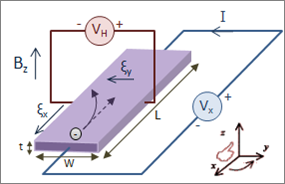
\includegraphics[width=70mm]{Images/fig1.png}
	\caption{نمودار کلی اثر هال 
\cite{noauthor_hall_2021}	
}\label{fig:hall}
\end{figure}

فرمول نیروی لورنتز به صورت 
\begin{equation}
	\boldsymbol{F} = q(\boldsymbol{E} + \boldsymbol{v} \times \boldsymbol{B})
\end{equation}
است.
\cite{halliday2010fundamentals}

با فرض سرعت در راستای $x$ و میدان مغناطیسی در راستای $z$ می‌دانیم که عبارت $v_x B_z$ به صورت منفی ظاهر خواهد شد. در حالتی که نیروی وارده صفر باشد، رابطه
\begin{equation}
0 = E_y - v_x B_z
\label{eq:2}
\end{equation}
را خواهیم داشت. البته باید توجه داشت که عملا به ازای الکترون‌ها،
$v_x\rightarrow -v_x$
و
$q \rightarrow -q$
است. $E_y$ همان میدان‌‌الکتریکی القایی است که منجر به ایجاد ولتاژ القایی اثرهال می‌شود.  در نتیجه از آن‌جایی که
$E_y = \frac{-V_H}{w}$
در نتیجه با جایگزینی در عبارت \eqref{eq:2} به رابطه
\begin{equation}
	V_H = v_x B_z w
	\label{eq:3}
\end{equation}
می‌رسیم.

با این وجود جریان قراردادی که عملا جریان حفره‌های حامل بار مثبت است، در خلاف جهت جریان الکترون‌ها و با بار منفی است، در نتیجه می‌توانیم برای جریان به رابطه
\begin{equation}
	I_x = ntw(-v_x)(-e)
\end{equation}
برسیم که در آن $n$ چگالی تعداد حاملین بار با واحد $m^{-3}$ است و $tw$ هم سطح مقطع عبوری را مشخص می‌کند. با حل معادله برحسب $w$ وجایگذاری آن در
\eqref{eq:3}
داریم \cite{noauthor_hall_2021}:
\begin{equation}
	V_H = \frac{I_x B_z}{n t e}.
\end{equation}


البته رایج است که در این رابطه ضریبی تحت نام ضریب هال به صورت 
\begin{equation}
	R_H = \frac{1}{n e}
\end{equation}
با واحد $m^3/C$ یا $\Omega cm/G$ تعریف کنند و رابطه نهایی به صورت
\begin{equation}
	V_H = R_H (\frac{I B}{t})
	\label{eq:7}
\end{equation}
نمایش داده می‌شود. در نتیجه عوامل اصلی در تعیین ولتاژ، شدت جریان، ضخامت ورقه و میدان مغناطیسی است.
\cite{ele_hall_2013}

نکته مهمی که در این روابط وجود دارد، این است که عملا جنس ذره حامل بار در آن اثر دارد. یعنی این که حامل جریان را الکترون فرض کردیم، در روابط بدست آمده اثرگذار بود. در نتیجه اگر فرض کنیم جهت میدان مغناطیسی برعکس شود، اثر برعکس بر الکترون‌ها گذاشته و منجر به تغییر علامت ولتاژ القایی می‌شود و از این طریق، می‌توانیم در جهت میدان مغناطیسی نیز تمایز قائل شویم.
\cite{noauthor_hall_2021}

نکته حائز اهمیت دیگر این است که  در عمل، بیش‌تر اوقات برای ورقه، از یک نیم‌رسانا استفاده می‌شود. دلیل این موضوع هم تاثیر گذاری همزمان الکترون‌ها و حفره‌ها در نیم‌رسانا است که باعث می‌شود ضرایب $R_H$ بزرگ‌تری بدست آمده و آشکارسازی ولتاژ به شکل راحت‌تری صورت بگیرد. برای نیم‌رسانا‌ها می‌توان در یک تقریب نسبتا خوب، $R_H$ را به صورت
\begin{equation}
	R_H = \frac{p \mu_h^2 - n \mu_e^2}{e(p\mu_h + n \mu_e)^2}
\end{equation}
بدست آورد که در آن، $n$ ضریب تجمع الکترون‌ها، $p$ ضریب تجمع حفره‌ها، $\mu_e$ تحرک‌پذیری الکتریکی الکترون‌ها و $\mu_h$ تحرک‌پذیری الکتریکی حفره‌ها و $e$ بار الکترون است. البته در چنین مواردی، حلیل نهایی تمامی روابط موجود به سادگی رابطه \eqref{eq:7} نیست اما آن رابطه می‌تواند دیدی سطح بالا و کلی از نحوه اثرگذاری پدیده هال به ما بدهد.
\cite{noauthor_hall_2021}


اگر بخواهیم به شکل  شهودی و مستقل از روابط ریاضیاتی به اثر هال نگاه کنیم، می‌توانیم آن را این طور توجیه کنیم که در اثر قرار گرفتن در میدان مغناطیسی، الکترون‌ها به جای عبور یک نواخت از نوار رسانا (نیم‌رسانا)، در یک سمت آن تجمع بیش‌تری پیدا کرده و در نتیجه آن حفره‌های مثبت در سمت دیگر تجمع خواهند کرد و به همین دلیل، اختلاف ولتاژ بین دو قسمت رسانا (نیم‌رسانا) ایجاد خواهد شد.


%\lr{SSIM}\LTRfootnote{ Structural SIMilarity (SSIM)}
%%%%%%%%%%%%%%%%%%%%%%%%%%%%%%% \section{شیوه‌ی پیشنهادی و نتایج}
\section{حسگر‌های مبتنی بر اثر هال}
\subsection{نحوه ساخت و طراحی مدار}
 
 نحوه کار کلی حسگر‌های مبتنی بر اثر هال، اساسا براساس تئوری توضیح داده شده در قسمت قبل است. عموما حسگرهای مبنتی بر اثر هال، از ورقه نازک مستطیلی شکلی از جنس نیم‌رسانای نوع \lr{P} نظیر گالیم آرسنید (\lr{GaAs})، ایندیم آنتیموان (\lr{InSb})،ایندیم آرسنید (\lr{InAs}) و یا ایندیم فسفید  (\lr{InP}) و البته در مواردی از گرافن که یکی از آلوتروپ‌های کربن و رسانا است، ساخته می‌شود که یک جریان به طور پیوسته در حال عبور از آن است. بر اثر تاثیرات مغناطیسی متغیر موردن اندازه‌گیری، اختلاف ولتاژی در دو سر این ورقه ایجاد می‌شود که به اندازه گیری این اختلاف ولتاژ و علامت آن، می‌توان به شدت این میدان مغناطیسی و همچنین جهت آن پی برد.
 \cite{wiki_sensor}
 

از خروجی این نوع حسگر‌ها هم در سیستم‌های خطی آنالوگ و هم در سیستم‌های دیجیتالی استفاده می‌شود. از آن جایی که عموما مقدار ولتاژ القایی بسیار کوچک و در حد میکروولت است، نیاز به تقویت کننده وجود دارد. در سیستم‌های آنالوگ، خروجی مستقیما وارد یک تقویت کننده عملیاتی شده و پس از آن به عنوان خروجی داده می‌شود. در سیستم‌های دیجیتالی این خروجی ممکن است وارد یک مبدل آنالوگ به دیجیتال شده و یا این که در بعضی سیستم‌ها که حالت روشن و خاموش دارند، وارد یک مقایسه‌گر اشمیت تریگر
\LTRfootnote{Schmitt Trigger (Hysteresis) Comparator}
 بشود. برای درک بهتر به شکل‌های
 \ref{fig:2}
 و
 \ref{fig:3}
  توجه کنید.
 
 \begin{figure}[t]
 	
 	\centering 
 	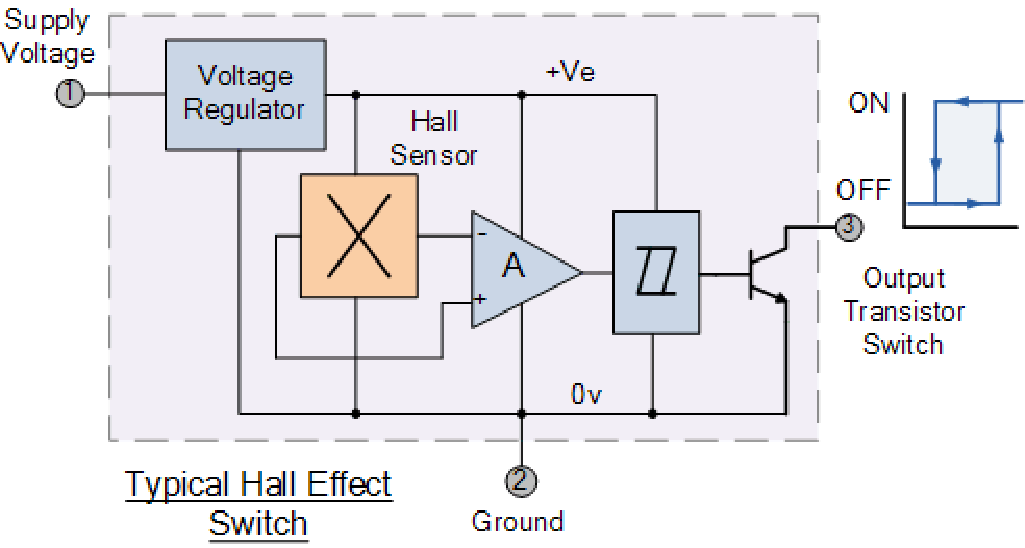
\includegraphics[width=70mm]{Images/2.pdf}
 	\caption{شمای کلی مدار اشمیت تریگر استفاده کننده از حسگر اثر هال. حسگر اثر هال با نماد مربعی که وسط آن ضربدر قرار دارد نمایش داده شده است. 
 		\cite{ele_hall_2013}	
 	}\label{fig:2}
 \end{figure}

\begin{figure}[t]
	
	\centering 
	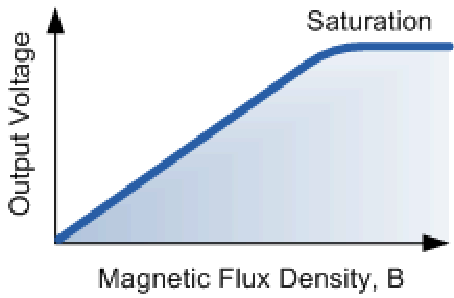
\includegraphics[width=50mm]{Images/3.pdf}
	\caption{نمودار کیفی خروجی ولتاژ حسگر آنالوگ نسبت به چگالی شار مغناطیسی عبوری. بعد از مقداری به بعد، به دلیل محدودیت تغذیه‌کننده تقویت کننده عملیاتی، ولتاژ به حالت اشباع می‌رسد.
		\cite{ele_hall_2013}	
	}\label{fig:3}
\end{figure}
 
 
دو نوع کلی سنسور دیجیتالی مبتنی بر اثر هال وجود دارد. دوقطبی و تک قطبی. در انواع دو قطبی، برای رفتن به حالت فعال نیاز به یک قطع مغناطیسی و برای رفتن به حالت غیرفعال نیاز به یک قطب مغناطیسی دیگر است. به بیان دیگر حدود مقایسه‌گر اشمیت‌ تریگر طوری تنظیم شده است که تنها با خروج از ناحیه میدان مغناطیسی، به حالت قبل بر نمی‌گردد. در نوع تک قطبی، تنها حضور یک قطب مغناطیسی برای فعال شدن و غیرفعال شدن کافیست و صرفا براساس خروج یا ورود به این میدان، امکان قطع و وصل خروجی نهایی وجود دارد.

نکته دیگری که وجود دارد این است که عموما خروجی جریان خیلی زیاد نبوده و در حدود $10$ تا $20$ میلی‌آمپر است. در نتیجه اگر لود مدار بالا باشد، یک حسگر معمولی شاید نتواند چندان خوب عمل کند و برای رفع این مشکل در مدار‌هایی که لود مقابل خروجی بزرگ است، یک ترانزیستور \lr{NPN} به صورت \lr{Open-Collector} به خروجی مدار اضافه می‌شود. 	\cite{ele_hall_2013}


\subsection{نحوه کارکرد}

از حسگر‌های مبتنی بر اثر هال، در بسیاری از مواقعی که نیاز به اندازه‌گیری نوعی حرکت و جابه‌جایی بدون برخورد مستقیم است، استفاده می‌شود. این حرکت و جا‌به‌جایی هم می‌تواند به صورت مستقیما رو به حسگر بوده و هم در جهت طرفین باشد. عموما جسمی که قرار است حرکت‌ آن اندازه‌گیری شود، ماهیتی فلزی داشته و با متصل کردن آهنربا به آن، خاصیت مغناطیسی در آن ایجاد می‌شود تا در اثر این میدان مغناطیسی، ولتاژی در حسگر مبتنی بر اثر هال ایجاد بشود.

\subsubsection{شناسایی حرکت رو به حسگر}

حرکت رو به حسگر یا \lr{Head-on} همان طور که مشخص است، نشان دهنده نزدیک یا دور شدن یک میدان مغناطیسی در جهت عمود بر حسگر است. در اثر دور یا نزدیک شدن یک جسم که خاصیتی مغناطیسی دارد، میدان و شار مغناطیسی گذرا از حسگر دچار تغییر شده و به همین دلیل، ولتاز‌های متفاوتی به عنوان خروجی داده می‌شوند که می‌توان از مقدار آن برای بدست آوردن فاصله جسم تا حسگر استفاده کرد.

از آن جایی که میدان مغناطیسی در نقطه‌ای مشخص با فاصله از منبع میدان نسبت عکس مجذوری دارد، عموما مدارهایی که خروجی حسگر را تحلیل می‌کنند و مثلا منجر به تغییر وضعیت یک چراغ و ورود آن به وضعیت روشن یا خاموش می‌شوند، ساختار غیرخطی دارند. برای درک بهتر این نوع کاربرد به شکل
\ref{fig:4}
توجه کنید.

\begin{figure}[t]
	
	\centering 
	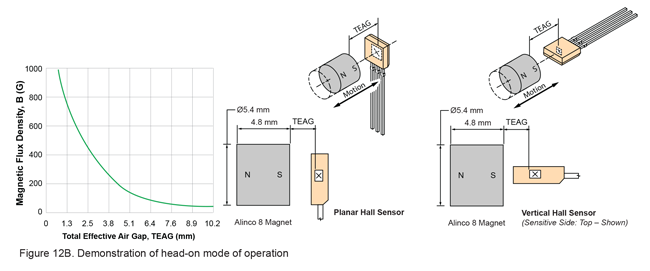
\includegraphics[width=75mm]{Images/head.png}
	\caption{حرکت رو به حسگر (\lr{Head-On}).
		معیار TEAG در نمودار بیانگر فاصله منبع مغناطیسی تا نزدیک‌ترین بخش قسمت فعال درون حسگر -یعنی همان ورقه اصلی سازنده آن- است.
		\cite{alleg}	
	}\label{fig:4}
\end{figure}

\subsubsection{شناسایی حرکت رو به طرفین}


روش دیگر استفاده از حسگر مبتنی بر اثر هال برای تشخیص حرکت به طرفین است. این شیوه به خصوص برای تشخیص میدان‌های مغناطیسی دوار و اندازه‌گیری سرعت چرخش موتور‌ها و سایر سیستم‌های چرخان موثر است.

بسته به نحوه قرارگیری میدان مغناطیسی، می‌توان تغییرات مثبت و منفی در ولتاژ را که می‌توانند ناشی از حرکات عمودی یا افقی باشند، تشخیص داد. برای درک بهتر این بخش به شکل
\ref{fig:5}
توجه کنید.

استفاده از این حسگر‌ها برای تشخیص سرعت چرخش موتور، خصوصا در کاربردهای مربوط به خودروسازی که حسگر در معرض آب، لرزش، روغن، گرد و خاک و عوامل دیگر قرار می‌گیرد، بدلیل عدم تاثیرگذاری جدی این موارد بر کارکرد حسگر و همچنین غیرتماسی بودن آن، بر حسگر‌های تماسی و همچنین حسگر‌های غیرتماسی دیگر نظیر حسگر‌های نوری ارجحیت دارد. \cite{ele_hall_2013}

	
\begin{figure}[t]
	
	\centering 
	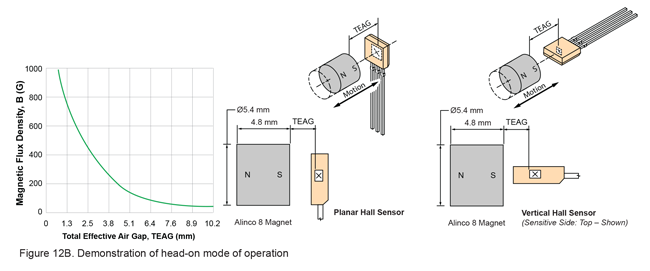
\includegraphics[width=75mm]{Images/side}
	\caption{حرکت رو به طرفین (\lr{Sideways}).
		معیار TEAG در نمودار بیانگر فاصله منبع مغناطیسی تا نزدیک‌ترین بخش قسمت فعال درون حسگر -یعنی همان ورقه اصلی سازنده آن- است.
		\cite{alleg}	
	}\label{fig:5}
\end{figure}


\subsubsection{حرکات آهنربا‌های مرکب}

اساس کار بعضی از این حسگرها، مبتنی بر وجود یک جفت آهنربا است که خود حسگر در میان آن‌ها قرار می‌گیرد. در یکسری از این حسگر‌ها قطب \lr{N} یک آهنربا در مقابل قطب \lr{S} آهنربای دیگر است که به این نوع حسگر‌ها، \lr{Push-Pull} گفته می‌شود. در نوع دیگر دو قطب همنام \lr{S} رو به روی هم قرار می‌گیرند و حسگر در میان‌آنا قرار می‌گیرد که به این نوع حسگر‌ها، \lr{Push-Push} گفته می‌شود. شکل‌های 
\ref{fig:6}
و
\ref{fig:7}
مربوط به این دو نوع هستند. \cite{alleg}



\begin{figure}[t]
	
	\centering 
	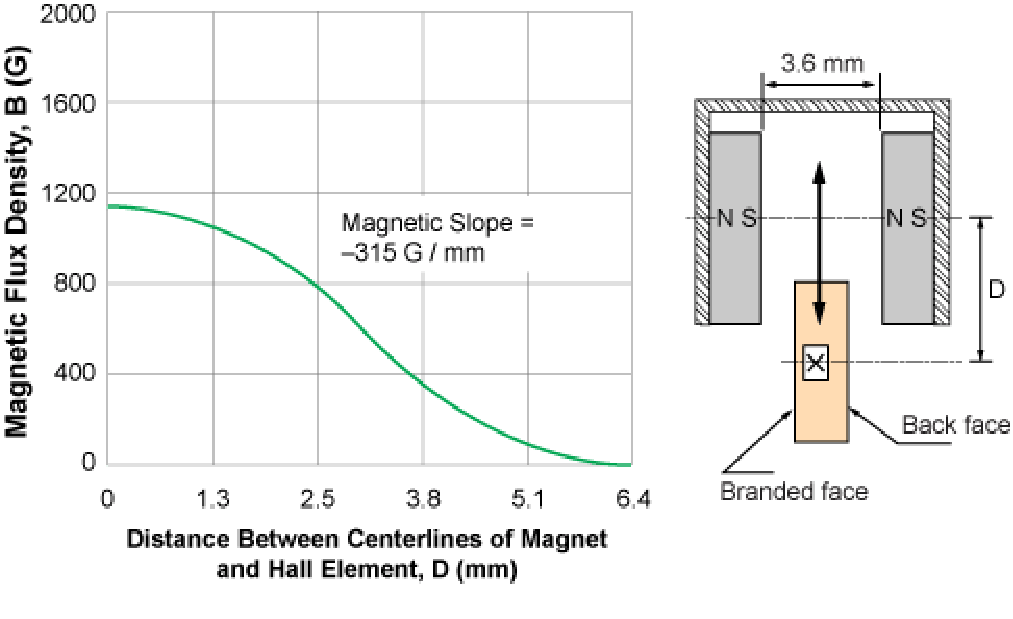
\includegraphics[width=75mm]{Images/7.pdf}
	\caption{حسگر نوع \lr{Push-Pull}. در این نوع، دو قطب ناهمنام آهنربا در دو طرف حسگر قرار می‌گیرند.
		\cite{alleg}	
	}\label{fig:6}
\end{figure}

\begin{figure}[t]
	
	\centering 
	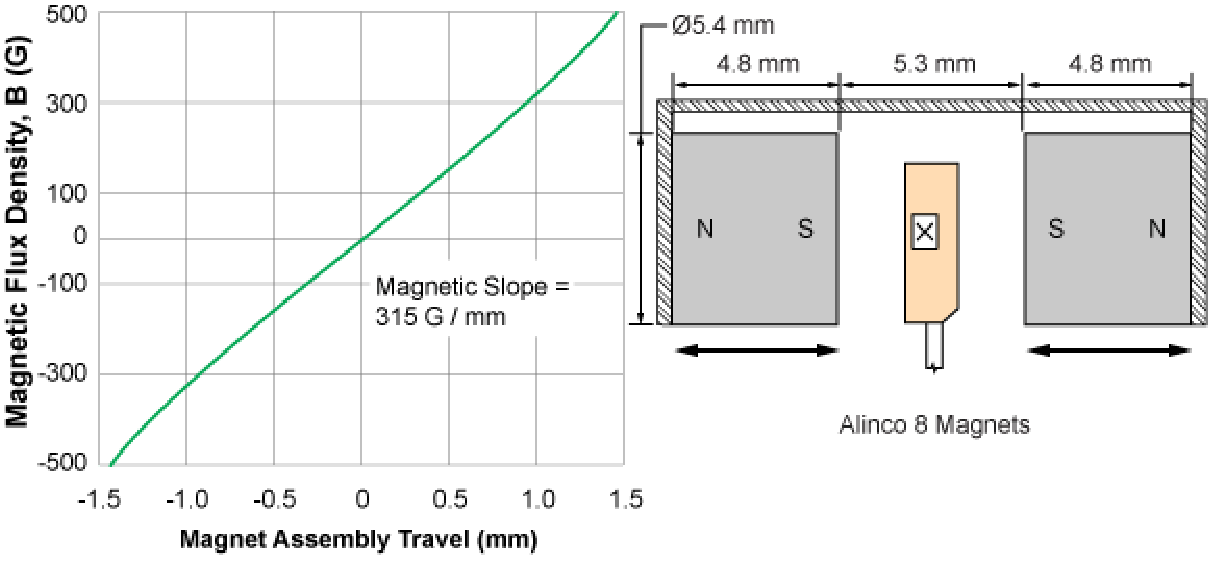
\includegraphics[width=75mm]{Images/8.pdf}
	\caption{حسگر نوع \lr{Push-Push}. در این نوع، دو قطب همنام \lr{S} آهنربا در دو طرف حسگر قرار می‌گیرند.
		\cite{alleg}	
	}\label{fig:7}
\end{figure}


\subsection{کاربردها، مزایا و معایب}

\subsubsection{کاربردها}
یکی از مهم‌ترین حوزه‌هایی که از حسگر‌های مبتنی بر اثر هال در آن استفاده می‌شود، صنعت خودروسازی است. 

یکی از کاربردهای حسگر‌های اثر هال در خودرو، اندازه‌گیری سطح سوخت است. در بعضی خودروها، آهنرباهای دائمی کوچکی درون مخزن سوخت قرار دارند که چگالی آن‌ها کمتر از سوخت بوده و با ورود سوخت به درون مخزن، بالا می‌آیند. در بالای مخزن، حسگر اثر هال قرار دارد و با نزدیک شدن این آهنرباها به آن، میدان مغناطیسی گذرنده از آن افزایش یافته و در نتیجه ولتاژ خروجی آن‌ هم افزایش می‌یابد و از این طریق سطح سوخت در مخزن مشخص می‌شود. \cite{rs}

کاربرد دیگر این حسگرها در سرعت‌سنج‌های خودرو 
\LTRfootnote{Tachometer}
است. این حسگر‌ها در نزدیکی اجزای چرخان ماشین نظیر شفت‌ها و چرخ‌ها نصب شده و به این اجزا نیز خاصیت آهنربایی داده می‌شود. از طریق شناسایی چرخش و حرکت رو به طرفین این قطعات نسبت به حسگر، میزان تعداد دور‌های چرخش آنان در دقیقه و به طبع آن سرعت خودرو تعیین می‌شود.  \cite{rs} به دلیل توانایی کنترل سرعت چرخش چرخ‌ها، در سیستم‌های ترمز ضدقفل
\LTRfootnote{ABS}
هم از این نوع حسگر‌ها استفاده می‌شود.
\cite{magnelink}

همچنین برای برخی از سیستم‌های ایمنی خودروها نظیر کنترل وضعیت صندلی، کنترل وضعیت بسته بودن کمربند ایمنی و همچنین تشخیص برخورد برای فعال‌سازی کسیه‌هوا هم از حسگرهای مبتنی بر اثرهال استفاده می‌شود. \cite{magnelink}

از آن‌جایی که این اجزا در ماشین در معرض برخورد آب، گرد و غبار و همچنین لرزش فراوان هستند، استفاده از این نوع حسگر‌ها نسبت به حسگر‌های تماسی و همچنین حسگر‌های نوری ارجحیت دارد. البته توجه کنید که با توجه به گستردگی صنعت خودروسازی، ممکن است برای موارد ذکر شده در بالا در بعضی خودروها از روش‌های دیگری استفاده شود ولی روش مبتنی بر حسگر‌های اثر‌ هال هم جزو روش‌های رایج است. 

صنعت دیگری که در آن از این حسگرها استفاده می‌شود، صنعت تولید گوشی‌های هوشمند و لپ‌تاپ است. برای بعضی از گوشی‌های هوشمند کاور‌های مغناطیسی وجود دارد که در اثر بسته شدن آن، باید صفحه گوشی خاموش بشود. این موضوع برای لپ‌تاپ‌ها هم صادق است و با بسته شدن درب، باید سیستم به وضعیت خواب برود و حداقل صفحه نمایش آن خاموش شود. در این سیستم‌ها از حسگرهای مبتنی بر اثر هال در وسیله استفاده می‌شود که با بسته شدن درب که خاصیت مغناطیسی دارد، ولتاژ خروجی حسگر افزایش یافته و این ولتاژ وارد یک مدار اشمیت تریگر می‌شود تا بعد از رسیدن به سطح مشخصی، سیگنال مربوط به خاموش کردن مشخص می‌شود. \cite{rs}

توجه کنید که لپ‌تاپ‌ها و همچنین گوشی‌های موبایل ممکن است با تغییرات دمای محسوسی از حدود دمای اتاق گرفته تا دمای نزدیک به $90\deg C$ مواجه شوند و در نتیجه استفاده از حسگر‌های غیرتماسی که نسبت به دما تغییر چشمگیری نداشته باشند، در این جا از اهمیت چشمگیری برخوردار است.

در سایر قسمت‌های صنایع مرتبط با الکترونیک هم از این حسگر‌ها استفاده می‌شود. سرعت چرخش دیسک‌های سخت
\LTRfootnote{Hard Drive Disk}
نیز به کمک این حسگر‌ها اندازه‌گیری می‌شود. همچنین کنترل مکانیزم زمان‌بندی در بعضی از دوربین‌ها هم از طریق این حسگرها با چرخاندن پیچ مربوط به زمان‌بندی، موقعیت یک منبع میدان مغناطیسی نسبت به حسگر تغییر کرده و با بازگشت آن به نقطه قبل، حسگر سیگنال مربوط به گرفتن عکس را تولید می‌کند.
\cite{magnelink}

علاوه بر این، در سیسیتم‌های مربوط به اتوماسیون امور روزمره هم از این حسگر‌ها استفاده می‌شود. در سیستم‌هایی نظیر سینک‌های ظرفشویی خودکار که با نزدیک شدن دست، باز می‌شوند، سیستم‌های خشک‌کن دست و همچنین درهای اتوماتیک هم از انواع دیجتیالی حسگر‌های مبتنی بر اثل هال استفاده شده است. البته بعضی از این سیستم‌ها از طریق سنسور‌های دیگر نظیر حسگر‌های نوری هم ساخته می‌شوند ولی انواع مبتنی بر حسگر اثر هال هم رایج است.
\cite{magnelink}

حتی در بسیاری از لوازم‌خانگی دیگر که شاید در نگاه اول چندان مرتبط به این نوع حسگر نباشند هم از آن‌ها استفاده شده است. در ماشین لباس‌شویی، جاروبرقی و همچنین ماشین ظرف‌شویی برای کنترل دور موتور از این نوع حسگر‌ها استفاده می‌شود. در ماشین لباس‌شویی علاوه بر کنترل دور موتور، سرعت چرخش محفظه درونی و همچنین سطح آب،‌از این سنسور‌ها برای تعیین تعادل ماشین لباس‌شویی هم استفاده می‌شود تا در اثر چرخش با سرعت بالا در جهت خاصی، سقوط نکند و در صورت خارج شدن از تعادل، سرعت کنترل بشود. در یخچال و همچنین اجاق‌برقی، حسگر‌های اثرهالی که براساس عناصر مغناطیسی موجود در درب کار‌ می‌کنند، با باز شدن در آن منجر به روشن شدن چراغ می‌شوند.
\cite{alleg2}


 
\subsubsection{مزایا}

اصلی ترین مزیت استفاده از حسگر‌های مبتنی بر اثر هال، عدم وابستگی فیزیکی آن‌ها به متغیر مورد اندازه‌گیری و کارکرد آن بدون نیاز به تماس است. در نتیجه این حسگرها دچار استهلاک نشده و عمر بسیار طولانی دارند و در نتیجه عملا نیاز به صرف هزینه برای نگهداری ندارند. \cite{ratna} این عدم برخورد فیزیکی، باعث می‌شود که در کابردهای با فرکانس بالا هم بتوان از این حسگر‌ها استفاده کرد، زیرا برخلاف حسگر‌های مکانیکی که در بسامدهای بالا تحت تنش زیادی قرار می‌گیرند، حسگر‌های مبتنی بر اثر هال دچار مشکل جدی نخواهند شد. \cite{wiki_sensor}

از طرف دیگر، در محیط‌های که گرد و خاک، آب، روغن لرزش زیاد وجود دارد، استفاده از سایر حسگر‌ها ممکن است با خطای زیادی همراه باشد چون این عناصر می‌توانند حسگر‌های تماسی و همچنین حسگر‌های غیرتماسی مبتنی بر نور را به شدت تحت تاثیر قرار بدهند. با این وجود،‌ این موارد بر روی حسگر‌های مبتنی بر اثر هال تاثیر بسیار اندکی می‌گذارند. \cite{wiki_sensor}

از طرف دیگر،  برخی دیگر از حسگرها که مبتنی بر میدان‌های مغناطیسی و القا هستند،‌ تنها توانایی اندازه گیری اختلاف و تفاضل را دارند. در حالی که از حسگر‌های مبتنی بر اثر هال می‌توان برای اندازه‌گیری میدان مغناطیسی به صورت مطلق و به صورت غیرتفاضلی هم استفاده کرد.  \cite{wiki_sensor}
 
 \subsubsection{معایب}
 
 با وجود مزایای بسیار،‌ این حسگرها معایبی هم دارند. با توجه به این که عموم میدان‌های مغناطیسی ساخته شده توسط آهنرباهای مصنوعی،‌ اندازه کمی دارند، عموما برای فواصل بیش از $10$ سانتی‌متر نمی‌توان از این حسگرها استفاده کرد. مگر این که از آهنرباهای فوق العاده قوی استفاده بشود که خود می‌توانند مخاطرات ایمنی جدی را به دنبال داشته باشد. \cite{ratna}
 
 وجود میدان‌های مغناطیسی سایر عناصر موجود در محیط و حتی برخی عناصر داخلی نظیر سیم‌پیچ‌ها می‌تواند بر دقت اندازه‌گیری اثرگذار باشد. خصوصا در مورد سیم‌های خود دستگاه که در مجاورت سنسور و فاصله کم قرار دارند، باید بررسی‌های لازم جهت کاهش اثر ناشی از آن‌ها و یا وارد کردن اثر آنان در محاسبات انجام بشود. \cite{ratna}
 
 دماهای خیلی بالا یا خیلی پایین می‌تواند تاثیر به شدت قابل توجهی بر مقاومت درونی ورقه مورد استفاده گذاشته \cite{ratna} و در نتیجه با تغییرات غیرخطی در مقاومت، دقت حسگر در این دماها به شدت پایین بیاید و حتی در بعضی موارد در اثر بالا رفتن بیش از اندازه مقاومت،‌ ممکن است ولتاژ القایی به قدری کم باشد که عملا امکان آشکارسازی آن با هزینه معقول وجود نداشته باشد.
 
\section{بررسی مختصر یک نمونه‌ حسگر  صنعتی}

با توجه به موارد گفته شده، این حسگرها کاربرد گسترده‌ای در صنعت دارند. با توجه به این موضوع، انواع مختلفی از آن‌ها در ابعاد و اشکال مختلف برای کاربردهای گوناگون تولید می‌شوند. عموم آن‌ها به صورت سه‌پایه هستند که دو پایه تغذیه و یک پایه خروجی است. برخی نمونه‌های چهارپایه هم وجود دارد که کاربردهای خاص خود را دارند. در این جا به طول خلاصه حسگر \lr{AH226}  ساخته شرکت \lr{Diodes Incorporated} را بررسی می‌کنیم.

این حسگر، به صورت چهارپایه است و از آن در موتورهای DC بدون جاروبک برای اندازه‌گیری میدان‌های مغناطیسی تولیدی بین سیم‌پیچ‌ها استفاده می‌شود. این حسگر به صورت دیجیتالی کار می‌کند. درون آن علاوه بر حسگر مبتنی بر اثل حال، یک تقویت کننده عملیاتی و یک مقایسه‌گر اشمیت تریگر هم قرار گرفته‌اند. علاوه بر این، چهارترانزیستور \lr{Open-Collection} با آرایش موسوم به \lr{Darlington} هم قرار گرفته‌اند تا امکان اتصال آن به خروجی با بار مقاومتی بالا فراهم بشود.



\section{جمع‌بندی}\label{Sec:Conclusion}
نویسندگان در شیوه‌ای جدید برای افزایش وضوح یک تصویر با استفاده از یک تصویر آموزشی ارائه نموده بودند که در مقاله‌ی حاضر به رفع مشکلاتی از آن پرداخته شد. استفاده از یک روش ثبت تصویر مبتنی بر ناحیه به منظور دقیق‌تر شدن مدل نگاشت تصاویر و حذف مرزهای تصاویر با یک روش همرنگ‌سازی بدون درز مراحلی هستند که در کار قبلی انجام نشده بودند. نوآوری اصلی این مقاله لحاظ کردن معیار شباهت ساختاری دو تصویر در فرمولبندی شیوه‌ی معروف ثبت تصویر لوکاس-کاناد و استفاده از آن در وضوح برتر می‌باشد. نتایج پیاده‌سازی‌های انجام شده برتری شیوه‌ی ثبت تصویر پیشنهادی و همچنین کارائی آنرا در مسأله‌ی وضوح برتر در مقایسه با برخی از دیگر روشها نشان داده است.

\subsection*{سپاس‌گزاری}
مؤلفین وظیفه‌ی خود می‌دانند که از آقای دکتر \lr{Peter Kovesi} بابت توابع سودمند \lr{MATLAB} 
و آقایان وفا خلیقی، مصطفی واحدی و دکتر مهدی امیدعلی بابت زحمات و راهنمایی‌های ارزنده‌ی آنها در زمینه‌ی
زی‌پرشین\RTLfootnote{زی‌پرشین با لوگوی \lr{\XePersian} بسته‌ی حروف‌چینی رایگان فارسی مبتنی بر \lr{\LaTeXe} 
و تحت سیستم‌عامل‌های ویندوز، لینوکس و مک
 می‌باشد:
 {\lr{http://www.parsilatex.com/\hfill}}} (که این مقاله با آن آماده شده است) تشکر به عمل آورند. 



%\begin{latin}
{
% سه دستور زیر باعث می‌شوند که مراجع با قلم کوچکتر و با فاصله خطوط کمتر و با فاصله بین مراجع کم ظاهر شوند. 
% این حالت برای کاهش تعداد صفحات مقاله مناسب است.
% می‌توانید هر یک از آنها را comment نموده و خروجی را ملاحظه فرمایید.
\small % این دستور الزامی نیست.
%\singlespacing
%\setlength{\itemsep}{-2ex}
%اگر از فایلهای سبک انگلیسی مانند latex8.bst یا IEEEtrans استفاده کنید بایستی کل قسمت مراجع را در داخل یک محیط latin قرار دهید (که در حال حاضر comment شده است و دستور زیر را نیز از حالت comment خارج کنید.
\renewcommand{\refname}{\rl{مراجع\hfill}}
\bibliographystyle{ieeetr-fa}%{IEEEtrans}%{latex8}%
\bibliography{References}
}
%\end{latin}

\end{document}